\documentclass[12pt]{article}

% --- Packages ---
\usepackage[margin=1in]{geometry}
\usepackage{amsmath,amssymb}
\usepackage{graphicx}
\usepackage{booktabs}
\usepackage{setspace}
\usepackage{hyperref}
\usepackage[round]{natbib}
\usepackage{url}
\usepackage{caption}
\usepackage{subcaption}
\usepackage{float}

% --- Dynamic statistics ---
% Auto-generated by 02_irt_model.R (bifactor) — do not edit by hand

\newcommand{\nLeaders}{497}
\newcommand{\nCountries}{123}
\newcommand{\nIndicators}{11}
\newcommand{\ecv}{12.5}

\newcommand{\fitMtwo}{36.15}
\newcommand{\fitDf}{33}
\newcommand{\fitPval}{0.3237}
\newcommand{\fitRMSEA}{0.0139}
\newcommand{\fitRMSEAlow}{0.0000}
\newcommand{\fitRMSEAhigh}{0.0366}
\newcommand{\fitSRMSR}{0.0448}
\newcommand{\fitTLI}{0.9949}
\newcommand{\fitCFI}{0.9969}
\newcommand{\fitAIC}{3410.83}
\newcommand{\fitBIC}{3549.72}
\newcommand{\fitLogLik}{-1672.42}

\newcommand{\thetaMean}{-0.000}
\newcommand{\thetaSD}{0.712}
\newcommand{\thetaMin}{-0.646}
\newcommand{\thetaMax}{2.403}

\newcommand{\discrimGTermLimitsAbsent}{1.098}
\newcommand{\discrimSTermLimitsAbsent}{3.478}
\newcommand{\discrimGPresidentForLife}{6.563}
\newcommand{\discrimSPresidentForLife}{11.244}
\newcommand{\discrimGFamilyInGovt}{1.040}
\newcommand{\discrimSFamilyInGovt}{-0.152}
\newcommand{\discrimGPlacesNamed}{1.475}
\newcommand{\discrimSPlacesNamed}{0.843}
\newcommand{\discrimGGrandioseTitles}{1.741}
\newcommand{\discrimSGrandioseTitles}{0.642}
\newcommand{\discrimGMonuments}{1.640}
\newcommand{\discrimSMonuments}{1.270}
\newcommand{\discrimGBirthdayHoliday}{2.283}
\newcommand{\discrimSBirthdayHoliday}{-0.229}
\newcommand{\discrimGHagiography}{1.475}
\newcommand{\discrimSHagiography}{1.431}
\newcommand{\discrimGCultOfPersonality}{6.353}
\newcommand{\discrimSCultOfPersonality}{5.465}
\newcommand{\discrimGCurrencyPortrait}{0.843}
\newcommand{\discrimSCurrencyPortrait}{0.068}
\newcommand{\discrimGOathToPerson}{2.986}
\newcommand{\discrimSOathToPerson}{24.541}

\newcommand{\topLeader}{Nkrumah}
\newcommand{\topCountry}{Ghana}
\newcommand{\topTheta}{2.403}

% Auto-generated by 04_gwf_comparison.R — do not edit by hand

\newcommand{\gwfNmatched}{351}
\newcommand{\gwfNpersonal}{156}
\newcommand{\gwfNnonpersonal}{195}
\newcommand{\gwfNunmatched}{146}
\newcommand{\gwfMeanPersonal}{0.111}
\newcommand{\gwfSDPersonal}{0.746}
\newcommand{\gwfMeanNonpersonal}{0.081}
\newcommand{\gwfSDNonpersonal}{0.756}
\newcommand{\gwfDiffMeans}{0.029}
\newcommand{\gwfPBr}{0.019}
\newcommand{\gwfPBp}{0.7168}
\newcommand{\gwfPBciLow}{-0.085}
\newcommand{\gwfPBciHigh}{0.124}
\newcommand{\gwfTstat}{-0.364}
\newcommand{\gwfTdf}{334.0}
\newcommand{\gwfTp}{0.7164}
\newcommand{\gwfCohensD}{0.039}
\newcommand{\gwfMeanNonPersonal}{0.081}
\newcommand{\gwfNNonPersonal}{195}
\newcommand{\gwfMeanHybridPersonal}{0.180}
\newcommand{\gwfNHybridPersonal}{61}
\newcommand{\gwfMeanPurePersonal}{0.066}
\newcommand{\gwfNPurePersonal}{95}
\newcommand{\gwfFstat}{0.497}
\newcommand{\gwfFp}{0.6085}


% --- Metadata ---
\title{Measuring Personalism in Dictatorships:\\A Latent Trait Approach with Observable Indicators}
\author{
  Lee Morgenbesser\thanks{[Affiliation TBD].} \and
  Charles Crabtree\thanks{Senior Lecturer, School of Social Sciences, Monash University and K-Club Professor, University College, Korea University. Email: charles.crabtree@monash.edu.}
}
\date{\today}

\begin{document}
\doublespacing

\maketitle

\begin{abstract}
\noindent How can we reliably measure the degree of personalism in dictatorships? Existing regime typologies classify personalist regimes categorically, yet personalism is better understood as a continuous, latent attribute that varies across leaders and over time. We introduce a new cross-national dataset covering \nLeaders{} authoritarian leader-spells in \nCountries{} countries (1946--present), coded on \nIndicators{} observable ``manifest'' indicators drawn from publicly available sources---constitutional texts, Wikidata, the Varieties of Democracy project, Wikipedia, and national currency records. We estimate a continuous personalism score for each leader-spell using a two-parameter Item Response Theory (IRT) model. The model achieves strong face validity: leaders widely regarded as highly personalist---including \topLeader{} (\topCountry{})---receive the highest scores, while leaders in institutionalised autocracies score near the bottom. We make the dataset, all code, and the interactive dashboard publicly available to facilitate future research on authoritarian politics.

\bigskip
\noindent\textbf{Keywords:} personalism, authoritarianism, measurement, Item Response Theory, dictatorships
\end{abstract}

\newpage

% ==========================================================================
\section{Introduction}
% ==========================================================================

How can we reliably measure the degree to which dictators have personalized political power? This question matters because personalist rule has profound consequences for governance, conflict, and regime survival \citep{geddes2014, weeks2014, svolik2012}. Despite its importance, existing measures of personalism suffer from weak measurement validity. Most influential datasets classify regimes into discrete categories---personalist, military, party, or monarchy---using expert judgments that are difficult to replicate and often disagree at the margins \citep{geddes2014, frantz2011}.

We propose an alternative approach. Rather than classifying regimes categorically, we treat personalism as a continuous, latent trait that can be inferred from observable indicators. Drawing on \citet{treier2008}'s application of Item Response Theory to measuring democracy, we compile \nIndicators{} binary indicators of personalism from publicly accessible data sources and estimate a latent personalism score ($\theta$) for \nLeaders{} authoritarian leader-spells across \nCountries{} countries.

% TODO: Add roadmap paragraph

% ==========================================================================
\section{Conceptualising and Measuring Personalism}
% ==========================================================================

% TODO: Morgenbesser's theoretical framework
% - Personalism as latent trait
% - Family resemblance structure: no single indicator necessary or sufficient
% - Two dimensions: power concentration and personality cult
% - Observable indicators as manifestations of the latent trait
% - Critique of existing categorical approaches (GWF, etc.)

\subsection{Existing Approaches}

% TODO: Review GWF, Wahman et al., Magaloni, etc.

\subsection{A Latent Trait Framework}

% TODO: Formal statement of the measurement framework
% - Why continuous > categorical
% - Why IRT > factor analysis for binary indicators with missingness

% ==========================================================================
\section{Data}
% ==========================================================================

We assemble data from five primary sources, compiling \nIndicators{} binary indicators for \nLeaders{} authoritarian leader-spells in \nCountries{} countries from 1946 to the present. Leader identification and tenure dates follow Archigos 4.1 \citep{goemans2009}.

\subsection{Indicators of Power Concentration}

Our power concentration indicators capture the extent to which the leader has subverted institutional constraints and centralised authority. From the Varieties of Democracy (V-Dem) dataset \citep{coppedge2024}, we extract dichotomised versions of expert-coded measures: political killings attributed to the state, military domination of the executive, judicial purges, constitutional disregard, and absence of legislative constraints. From the Constitute Project \citep{constitute}, we code whether constitutional term limits are absent and whether the constitution designates the leader as president for life. From Wikidata, we identify leaders who have placed family members in senior government positions.

\subsection{Indicators of Personality Cult}

Personality cult indicators capture the symbolic elevation of the leader. From Wikidata, we identify places named after leaders, grandiose titles, commissioned monuments, state-mandated birthday holidays, and state hagiographies. From Wikipedia, we flag leaders with documented cults of personality. From national currency records, we code whether the leader's portrait appears on banknotes during their tenure. From the Constitute Project, we code whether oaths of loyalty are directed to the leader personally rather than to the constitution.

% TODO: Coverage discussion, refer to Figure~\ref{fig:coverage}

\begin{figure}[H]
  \centering
  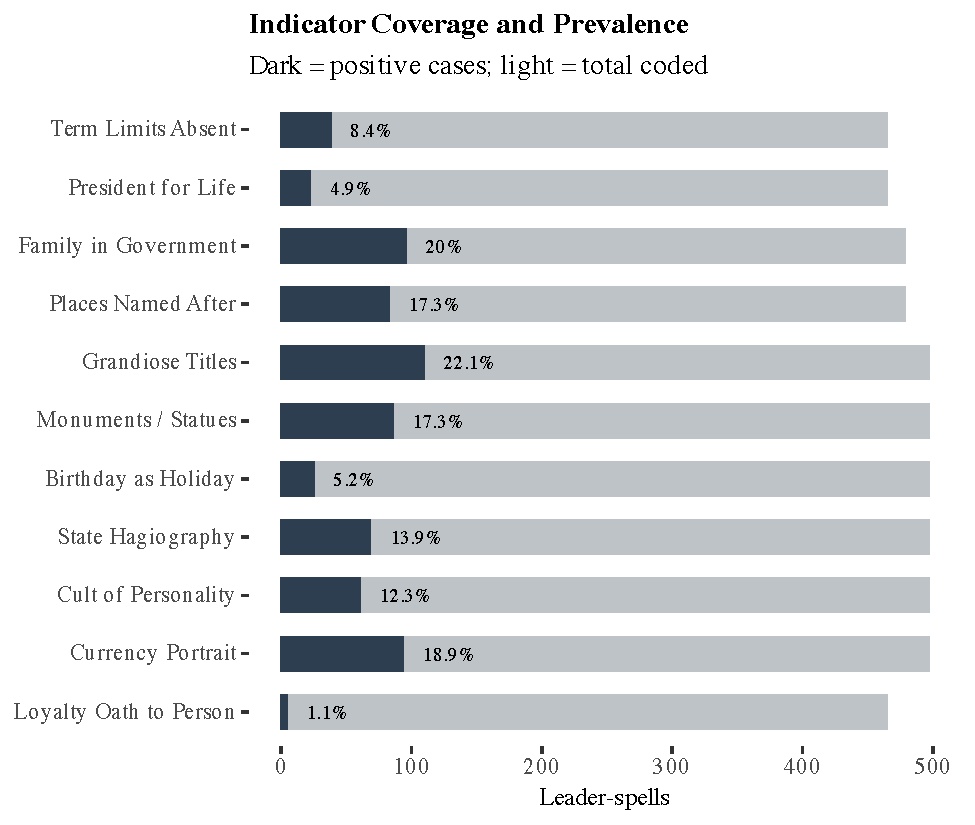
\includegraphics[width=\textwidth]{../figures/fig_coverage.pdf}
  \caption{Coverage and prevalence of the \nIndicators{} manifest indicators. Dark bars indicate positive codings; light bars show total coded cases.}
  \label{fig:coverage}
\end{figure}

% ==========================================================================
\section{Methods}
% ==========================================================================

We estimate a unidimensional two-parameter logistic (2PL) Item Response Theory model \citep{deayala2009, embretson2000}. For leader-spell $i$ and indicator $j$:

\begin{equation}
  P(Y_{ij} = 1 \mid \theta_i) = \frac{1}{1 + \exp\bigl(-a_j(\theta_i - b_j)\bigr)}
\end{equation}

\noindent where $\theta_i$ is the latent personalism score, $a_j$ is the discrimination parameter (how strongly indicator $j$ relates to personalism), and $b_j$ is the difficulty parameter (the level of personalism at which the indicator becomes more likely than not). Parameters are estimated via marginal maximum likelihood with the EM algorithm using the \texttt{mirt} package in R \citep{chalmers2012}. Missing values are handled natively under the assumption that they are missing at random.

Latent scores are estimated using Expected A Posteriori (EAP) estimation with associated standard errors, following \citet{treier2008}.

% ==========================================================================
\section{Results}
% ==========================================================================

\subsection{Item Parameters}

Figure~\ref{fig:item_params} displays the estimated discrimination and difficulty parameters for all \nIndicators{} indicators.

% TODO: Discuss which items are most discriminating and what this means substantively

\begin{figure}[H]
  \centering
  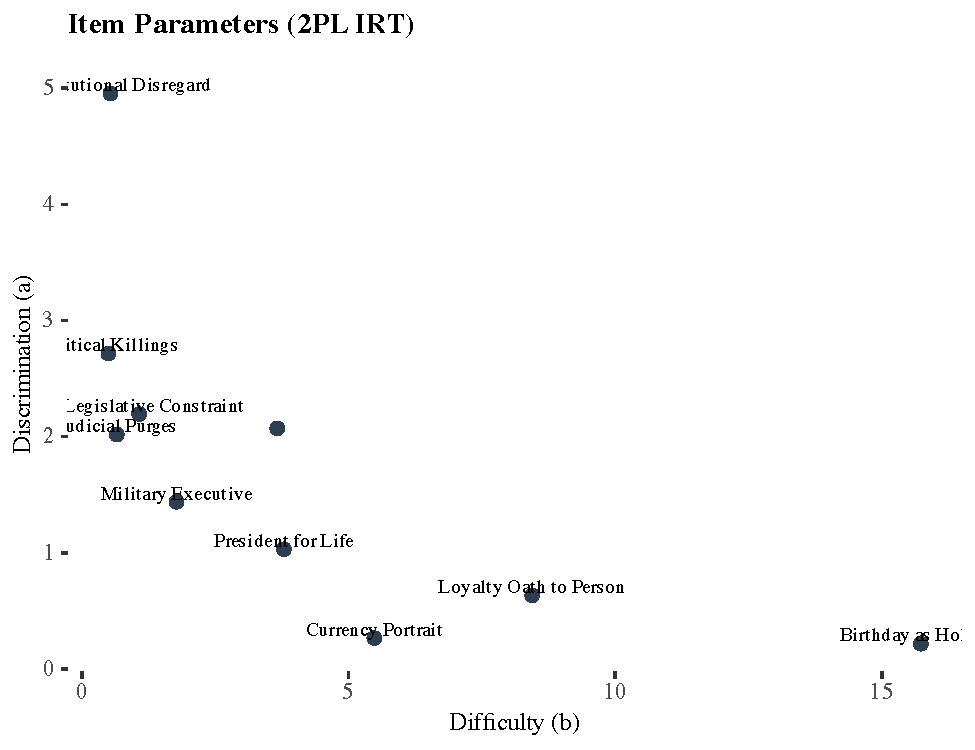
\includegraphics[width=\textwidth]{../figures/fig_item_parameters.pdf}
  \caption{Estimated item parameters from the 2PL IRT model. Discrimination ($a$) reflects how strongly each indicator relates to the latent personalism trait; difficulty ($b$) reflects the level of personalism required for the indicator to be more likely present than absent.}
  \label{fig:item_params}
\end{figure}

\subsection{Personalism Scores}

The distribution of estimated personalism scores ($\hat{\theta}$) is shown in Figure~\ref{fig:theta_dist}. Scores have a mean of \thetaMean{} (SD = \thetaSD{}), ranging from \thetaMin{} to \thetaMax{}.

\begin{figure}[H]
  \centering
  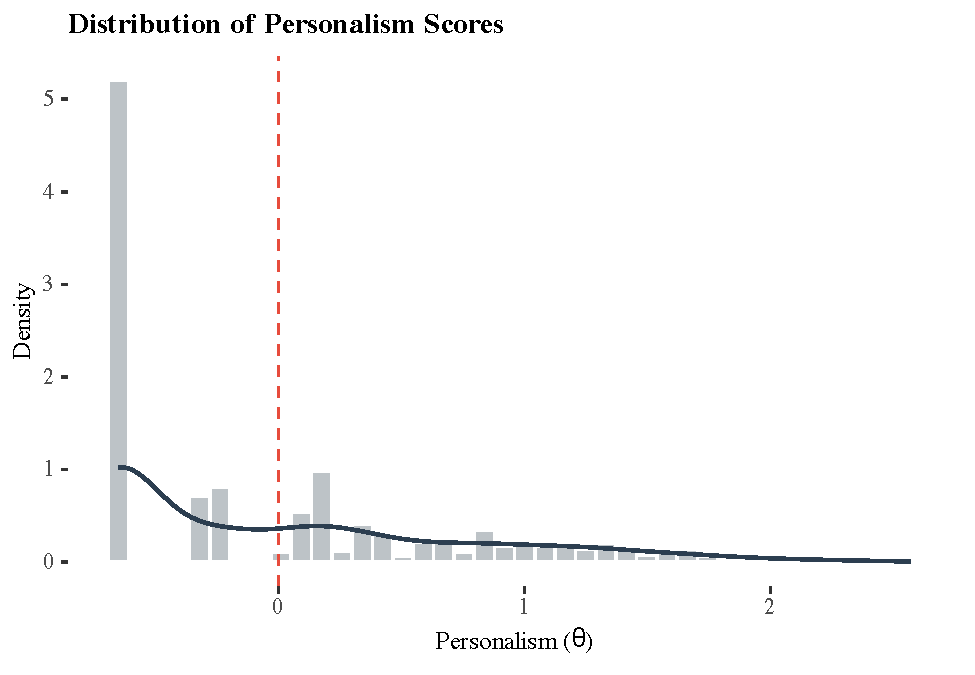
\includegraphics[width=\textwidth]{../figures/fig_theta_distribution.pdf}
  \caption{Distribution of estimated personalism scores ($\hat{\theta}$) across \nLeaders{} leader-spells. The dashed line indicates the mean.}
  \label{fig:theta_dist}
\end{figure}

\subsection{Face Validity}

Figure~\ref{fig:top_leaders} presents the 25 leaders with the highest estimated personalism scores. The ranking provides strong face validity: leaders widely regarded as highly personalist---such as \topLeader{} (\topCountry{})---occupy the top positions.

\begin{figure}[H]
  \centering
  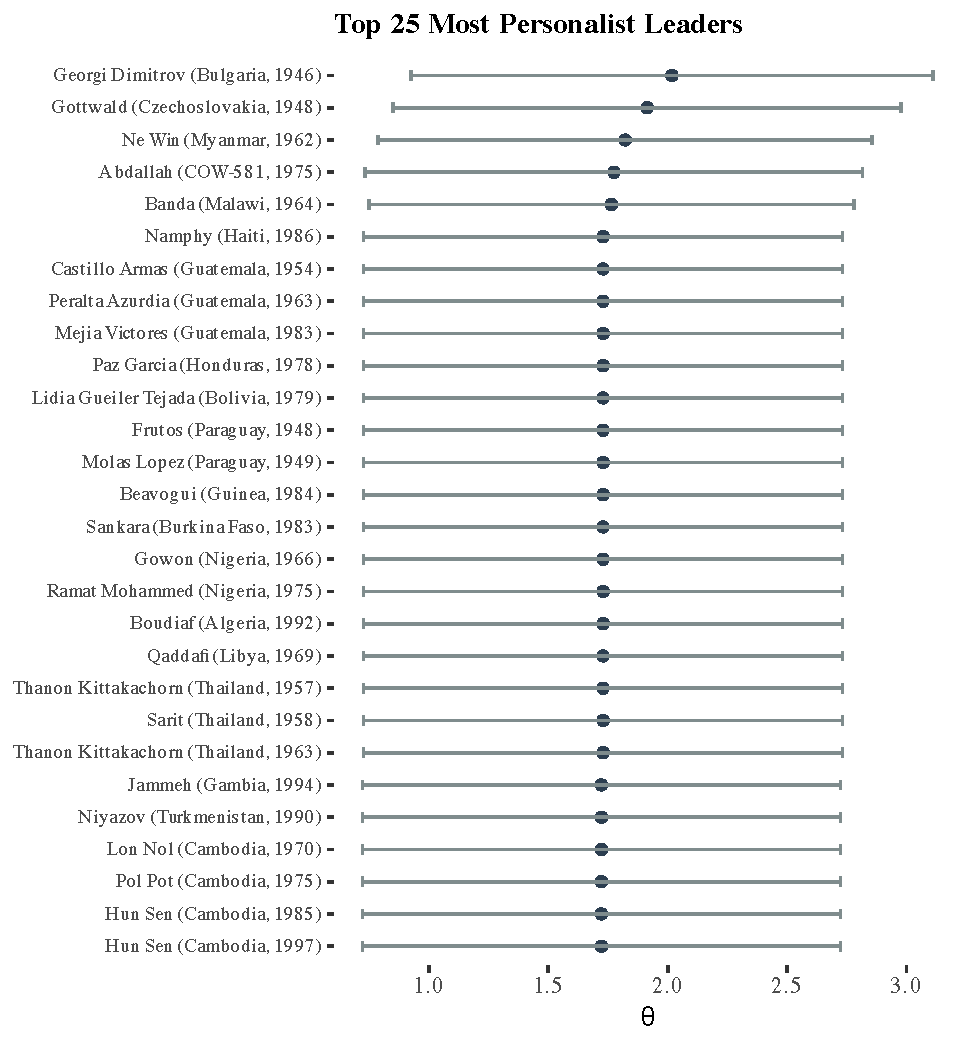
\includegraphics[width=\textwidth]{../figures/fig_top_leaders.pdf}
  \caption{The 25 leaders with the highest estimated personalism scores, with 95\% confidence intervals.}
  \label{fig:top_leaders}
\end{figure}

\subsection{Test Information}

Figure~\ref{fig:test_info} displays the test information function. The measure provides the most information---and therefore the most precise estimates---in the range of $\theta$ where personalism transitions from moderate to high levels.

\begin{figure}[H]
  \centering
  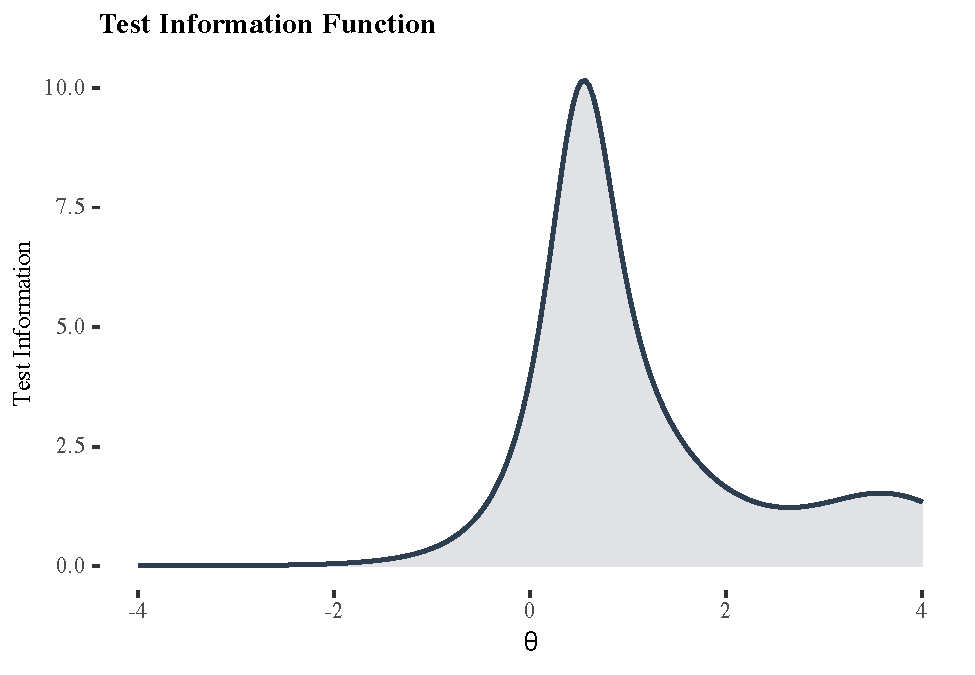
\includegraphics[width=\textwidth]{../figures/fig_test_information.pdf}
  \caption{Test information function. Higher values indicate greater measurement precision at that level of $\theta$.}
  \label{fig:test_info}
\end{figure}

\subsection{Model Fit}

% TODO: Discuss M2 fit statistic, RMSEA, CFI, TLI from statistics.tex macros
% The model yields RMSEA = \fitRMSEA{} [90\% CI: \fitRMSEAlow{}, \fitRMSEAhigh{}], CFI = \fitCFI{}, TLI = \fitTLI{}.

\subsection{Comparison with GWF Classifications}

As an external validation exercise, we compare our continuous personalism scores with the categorical regime classifications from \citet{geddes2014}. Of \nLeaders{} leader-spells, \gwfNmatched{} can be matched to GWF regime-years by COW code and temporal overlap; \gwfNunmatched{} remain unmatched, primarily because they govern after GWF coverage ends in 2010. Among matched leaders, \gwfNpersonal{} govern regimes classified as containing a personal element (``personal,'' ``party-personal,'' ``military-personal,'' or ``party-personal-military'') and \gwfNnonpersonal{} govern non-personal regimes.

Figure~\ref{fig:gwf_binary} displays the distribution of $\hat{\theta}$ by GWF binary classification. Leaders in personal regimes score marginally higher ($\bar{\theta}$ = \gwfMeanPersonal{}, SD = \gwfSDPersonal{}) than those in non-personal regimes ($\bar{\theta}$ = \gwfMeanNonpersonal{}, SD = \gwfSDNonpersonal{}), but the difference is small and not statistically distinguishable from zero (point-biserial $r$ = \gwfPBr{}, $p$ = \gwfPBp{}; Cohen's $d$ = \gwfCohensD{}; Welch $t$ = \gwfTstat{}, $p$ = \gwfTp{}).

The weak association is substantively informative. GWF classifies \textit{regimes}, while our measure captures \textit{individual-level} personalism across multiple observable dimensions, including personality cult indicators that GWF does not directly code. A leader may exhibit strong personalist tendencies---accumulating titles, naming places, commissioning statues---within a regime that GWF categorises as party-based or military. Conversely, some leaders in GWF-designated personal regimes may inherit personalist institutional structures without cultivating personality cults. This conceptual divergence supports our argument that personalism is better understood as a continuous, multidimensional trait than as a categorical regime property.

\begin{figure}[H]
  \centering
  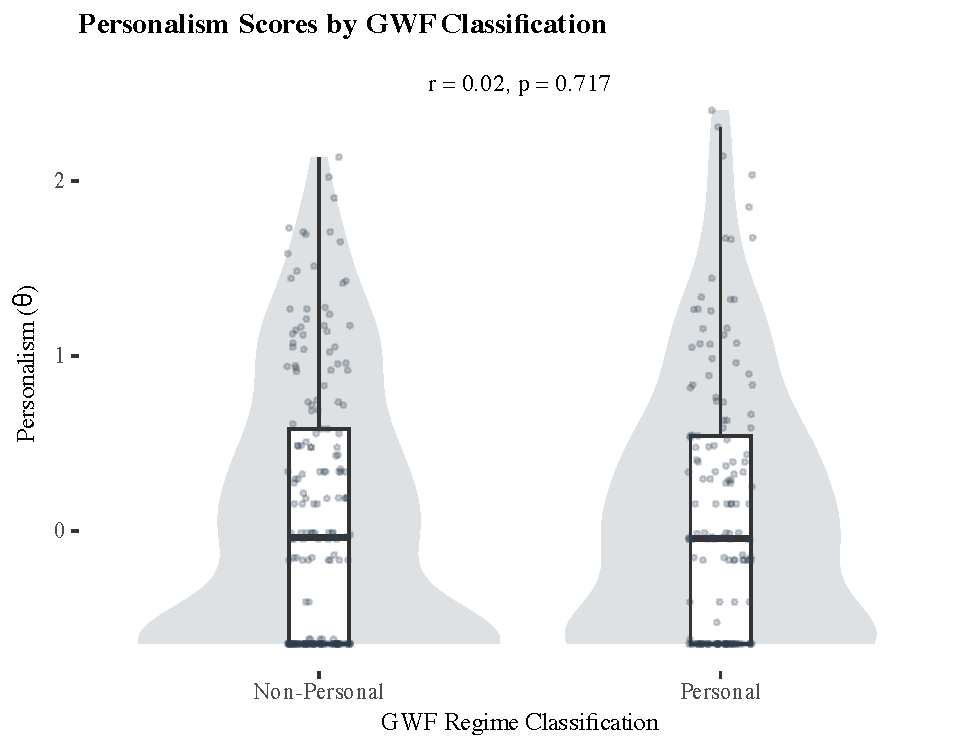
\includegraphics[width=\textwidth]{../figures/fig_gwf_binary.pdf}
  \caption{Distribution of personalism scores ($\hat{\theta}$) by GWF regime classification. ``Personal'' includes all GWF types containing a personal element. Boxes show interquartile ranges; violin contours show kernel density estimates.}
  \label{fig:gwf_binary}
\end{figure}

% ==========================================================================
\section{Discussion}
% ==========================================================================

% TODO: Substantive discussion
% - What do the item parameters tell us about the structure of personalism?
% - Are power concentration and personality cult empirically separable?
% - Applications: personalism as IV/DV in conflict, governance, transition research

\subsection{Limitations}

% TODO:
% - Survivorship bias in sources (prominent regimes better documented)
% - Monarchies: some indicators (currency, holidays) are standard practice
% - Temporal precision: indicators change infrequently
% - Low-prevalence items (cult_of_personality, oath_to_person) have weak discrimination
% - Unidimensional assumption may not hold

\subsection{Extensions}

% TODO:
% - Multidimensional IRT separating power concentration from personality cult
% - Dynamic IRT for time-varying personalism within leader-spells
% - Additional indicators from text mining (State Dept reports, GDELT)

% ==========================================================================
\section{Conclusion}
% ==========================================================================

% TODO: Brief conclusion restating contributions

% ==========================================================================
% Data Availability
% ==========================================================================
\bigskip
\noindent\textbf{Data Availability.} We will make all data and code used to generate our results available at a figshare repository at the time of publication.

% ==========================================================================
% Acknowledgments
% ==========================================================================
\bigskip
\noindent\textbf{Acknowledgments.} [TBD]

% ==========================================================================
% References
% ==========================================================================
\newpage
\bibliographystyle{apalike}
\bibliography{references}

% ==========================================================================
% Appendix
% ==========================================================================
\newpage
\appendix
\section{Item Characteristic Curves}

\begin{figure}[H]
  \centering
  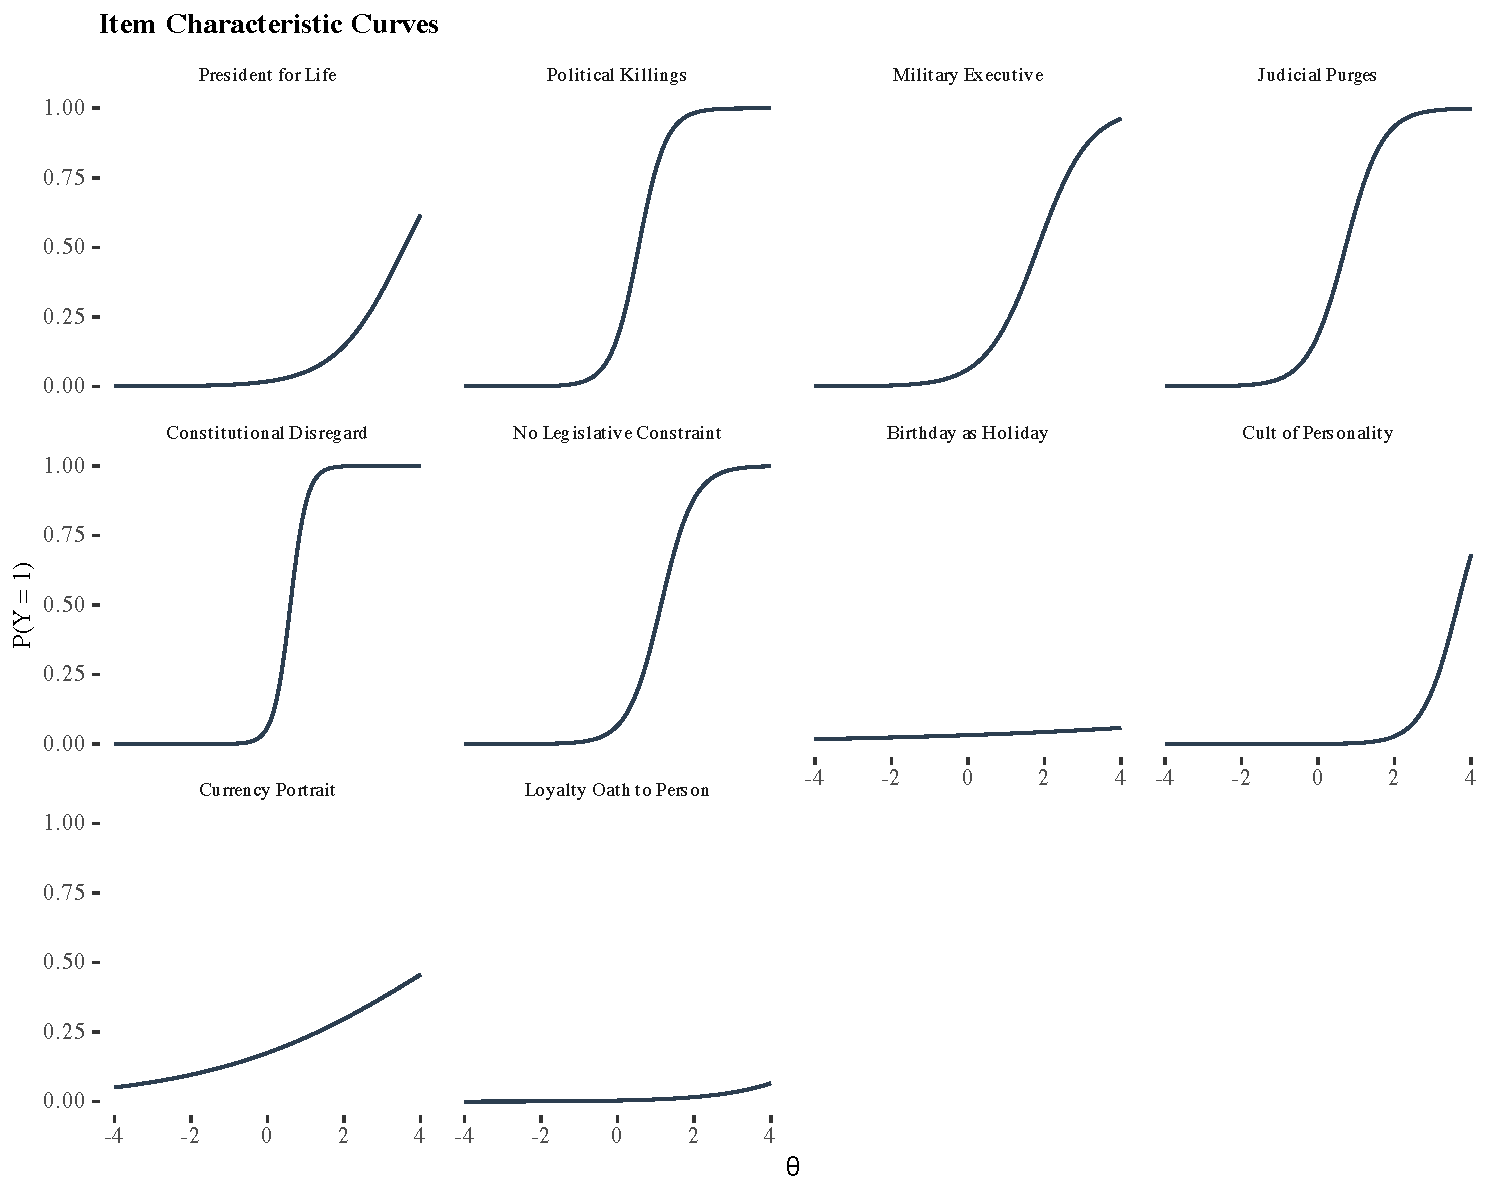
\includegraphics[width=\textwidth]{../figures/fig_icc_curves.pdf}
  \caption{Item Characteristic Curves (ICCs) for all \nIndicators{} indicators, showing the probability of a positive coding as a function of the latent personalism score $\theta$.}
  \label{fig:icc}
\end{figure}

\section{Bottom-Ranked Leaders}

\begin{figure}[H]
  \centering
  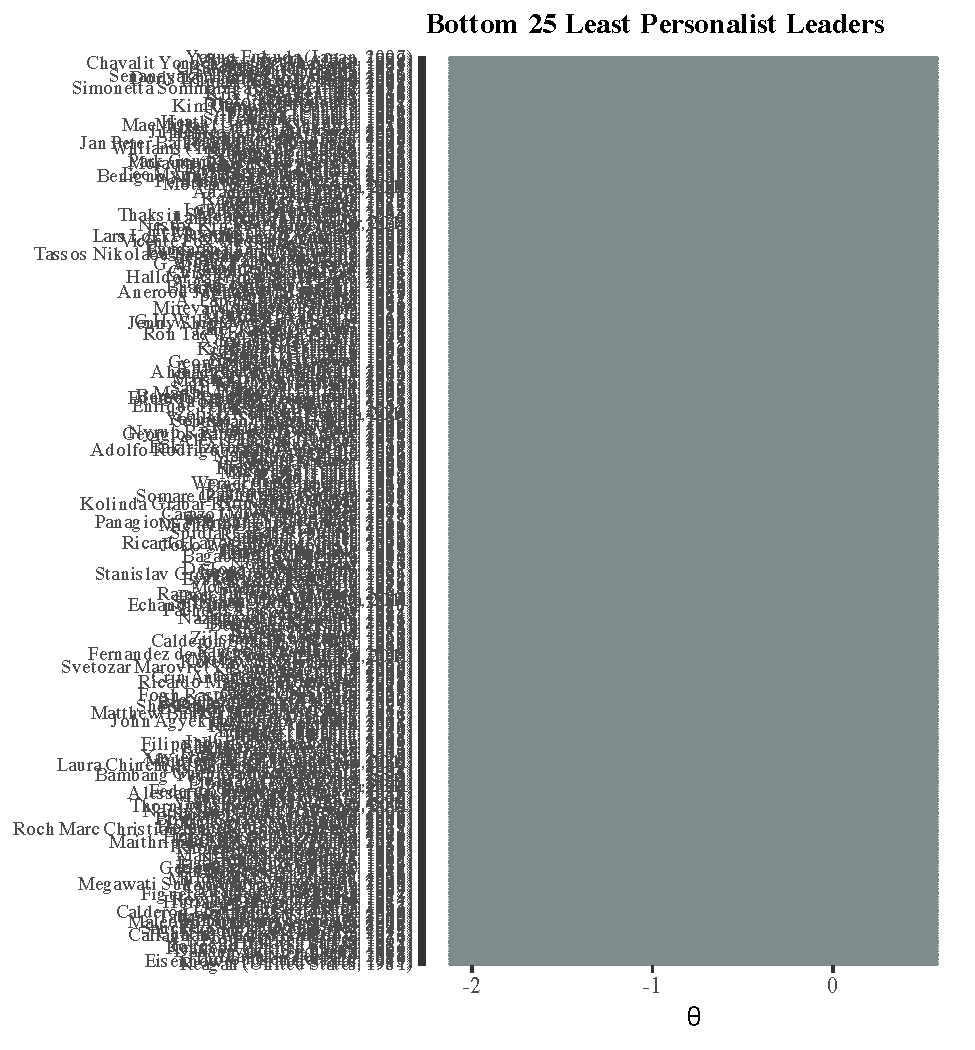
\includegraphics[width=\textwidth]{../figures/fig_bottom_leaders.pdf}
  \caption{The 25 leaders with the lowest estimated personalism scores, with 95\% confidence intervals.}
  \label{fig:bottom_leaders}
\end{figure}

% TODO: Add item fit statistics table
% TODO: Add full indicator coding table in appendix

\end{document}
